\subsection{Diseño de muros de corte o placas}
\subsubsection{Diseño a flexocompresión}
La cuantía mínima según el artículo 11.10.10.3: $\rho_{\mathrm{v}}=0.0025$\\
Para el muro en estudio de espesor 25cm se colocara en el alma doble malla de 3/8"@20cm lo que representa una cuantía de:
\FPset\svwall{20}
\FPset\ewall{25}
\FPset\asvwall{0.71}
\FPset\nfvwall{2}
\FPeval\pvwall{round(2*\asvwall/(\ewall*\svwall),4)}
\begin{align*}
\rho_{v} =\frac{n\cdot A_{sh}}{e\cdot s}=\frac{\nfvwall\cdot \asvwall}{\ewall\cdot \svwall}=\pvwall
\end{align*}
\noindent
Donde:\\
$e$: Espesor del muro\\
$\rho_{v}$: Cuantía vertical en el muro\\
$A_{sh}$: Área de la varilla utilizada\\
$n$: numero de capas\\
$s$: separación del refuerzo.\\
En el borde izquierdo de espesor constante se coloco 6 $\phi$ 5/8" en una longitud de 30cm, en el borde derecho que también funciona como una columna de 25x65cm se coloco una cuantía de 1\% haciendo un total de 10 $\phi$ 5/8", con el armado propuesto se hace la verificación en flexocompresión: 
\begin{figure}[h!]
    \centering
    \caption{Diagrama de interacción del muro PL-1}
    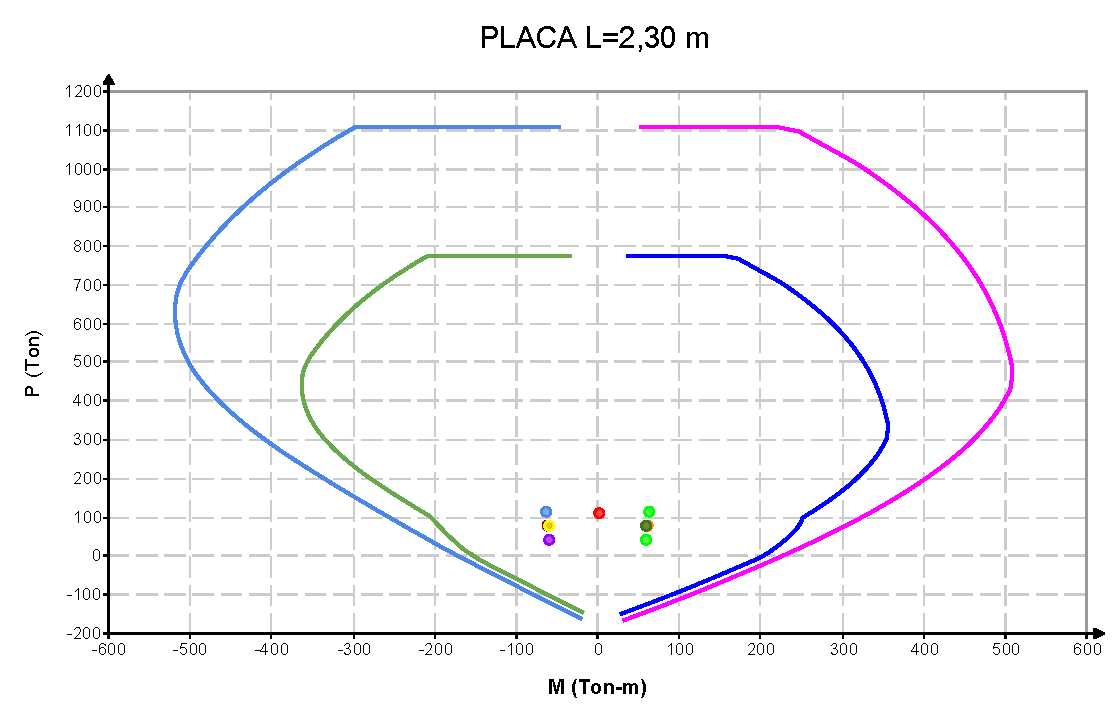
\includegraphics[scale=0.67]{IMAGENES/pl2.pdf}
    %\caption*{\small Fuente: \it \cite{E-060}}
    \label{atrans}
\end{figure}

\FPset\agwall{6750}
\FPeval{\limwall}{round(0.1*\fc*\agwall/1000,2)}
\noindent El limite de carga axial es:
\begin{align*}
0.1\;f_{c}^{'}\;A_{g}=0.1\cdot\fc\cdot\agwall=\limwall\mathrm{~ton}
\end{align*}
Las cargas ultimas amplificadas están por debajo de este valor por lo que no seria necesario las verificaciones que se mencionan a continuación para muros en flexocompresión.
\subsubsection{Diseño de elementos especiales de borde}
Los elementos de borde en la zona en compresión deben ser confinados cuando la profundidad del eje neutro exceda:
\begin{align}
c \geq \frac{l_{m}}{600\left(\delta_{u} / h_{m}\right)}  
\end{align}
\noindent
Según el artículo 21.9.7.4 este criterio solo aplica para muros continuos y diseñados para tener una sola sección critica para flexión y carga axial.\\
Si se requiere elementos de borde especiales la separación máxima $s_{0}$ dentro del núcleo confinado según 21.9.7.6 (e) será el menor de:
\begin{enumerate}
\item[] (a): $10 d_{b}$
\item[] (b): $\min \left(e, l_{c}\right)$
\item[] (c): $25 \mathrm{~cm}$
\end{enumerate}
\noindent
La longitud del elemento de borde debe cumplir con 21.9.7.6 (a) y no será menor que:
\begin{enumerate}
\item[] (a): $c/2$
\item[] (b): $c-0,1 \cdot l_{m}$
\end{enumerate}
La altura de confinamiento debe cumplir con 21.9.7.4 y no será menor del mayor valor obtenido con:
\begin{enumerate}
\item[] (a): $l_{m}$
\item[] (b): $ \displaystyle\frac{M_{u}}{4 \cdot V_{u}}$
\end{enumerate}
\noindent
Donde no se requiera elementos de borde confinados se debe cumplir con 21.9.7.7:\\
\noindent
La separación máxima del refuerzo transversal no deberá exceder 16 veces el diámetro de la barra longitudinal, 48 veces el diámetro del estribo y la menor dimensión del elemento en compresión.
\begin{enumerate}
\item[] (a): $16 d_{b}$
\item[] (b): $48 d_{e}$
\item[] (c): $\min (b, h)$
\item[] (d): $25 \mathrm{~cm}$
\end{enumerate}

\begin{figure}[h!]
    \centering
    \caption{Elemento especial de borde}
    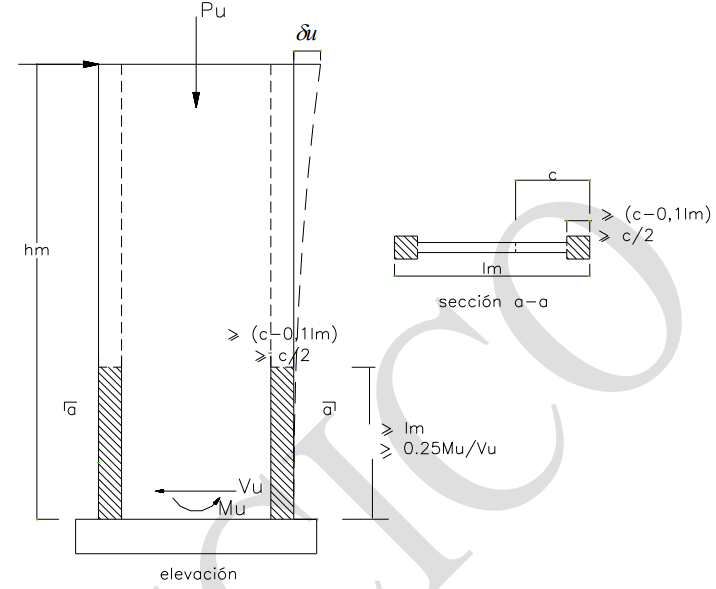
\includegraphics[scale=0.67]{IMAGENES/pl1.PNG}
    %\caption*{\small Fuente: \it \cite{E-060}}
    \label{atrans}
\end{figure}

En cualquier caso, los estribos deberán cumplir con:
\begin{itemize}
  \item Ninguna barra longitudinal esté separada a más de $150 \mathrm{~mm}$ libres de una barra apoyada lateralmente. (figura 13)

  \item El refuerzo transversal debe disponerse mediante estribos cerrados de confinamiento sencillos o múltiples. Se pueden usar grapas suplementarias del mismo diámetro de barra y con el mismo espaciamiento que los estribos cerrados de confinamiento.

  \item La distancia, centro a centro, transversal al eje del elemento, entre las ramas de estribos cerrados de confinamiento múltiples o entre las grapas suplementarias, hx, no deben exceder 350 mm medidos centro a centro.

\end{itemize}

\begin{figure}[h!]
    \centering
    \subfigure[]{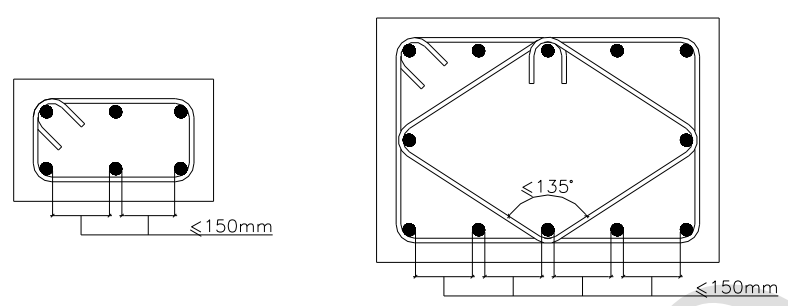
\includegraphics[width=100mm]{IMAGENES/est2.PNG}}\hspace{0mm}
    \subfigure[]{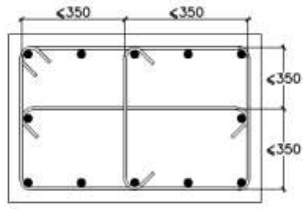
\includegraphics[width=50mm]{IMAGENES/est1.PNG}}
    \caption{Requisitos en estribos}
    \label{reqv}
\end{figure}

\subsubsection{Diseño a cortante}

\noindent Peralte efectivo del muro (Art. 21.9.4.5)
\begin{align}
    d=0,80 \cdot l_{w}
\end{align}
Contribución del concreto a cortante (Art. 11.10.5)
\begin{align}
   V_{c}=A_{c w} \cdot\left(\alpha_{c} \cdot \sqrt{f_{c}^{\prime}}\right)
\end{align}
\noindent
Donde:\\
$A_{c w}:$ Área resistente a cortante (área del alma) $A_{c w}=d \cdot e$\\
$e:$ Espesor del muro Donde $\alpha_{c}$ depende de la esbeltez del muro según:
\begin{align*}
&\alpha_{c} \text { es } 0,80 \text { para } \frac{h_{m}}{l_{w}} \leq 1,5 ; \\
&\alpha_{c} \text { es } 0,53 \text { para } \frac{h_{m}}{l_{w}}>2 \\
&\alpha_{c} \text { varia linealmente entre } 0,80 \text { y } 0,53 \text { para } \frac{h_{m}}{l_{w}} \text { entre } 1,5 \text { y } 2,0.
\end{align*}

\begin{figure}[h!]
    \centering
    \subfigure[]{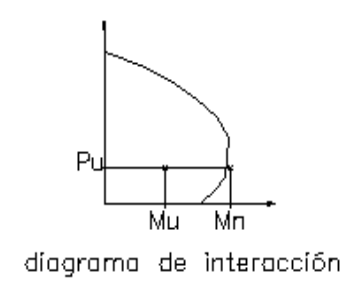
\includegraphics[width=65mm]{IMAGENES/wall2.PNG}}\hspace{10mm}
    \subfigure[]{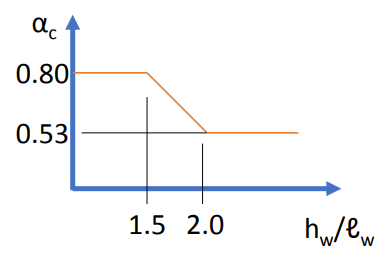
\includegraphics[width=75mm]{IMAGENES/walls.PNG}}
    \caption{Diseño a cortante de muros}
    \label{corw}
\end{figure}

Cortante máxima según el Art. 11.10.4
\begin{align}
    V_{n} \leq 2,6 \cdot \sqrt{f_{c}^{\prime}} \cdot A_{c w}
\end{align}
Cortante máxima en los estribos según la Ecu. 11-2
\begin{align}
    V_{s, \max }=V_{n}-V_{c}
\end{align}
Cortante requerida en estribos según la Ecu. 11-1
\begin{align}
    V_{s, r e q}=\frac{V_{u}-\phi_{c} \cdot V_{c}}{\phi_{c}}
\end{align}
Resistencia a corte del refuerzo horizontal según la Ecu. 11-31
\begin{align}
    V_{s}=A_{c w} \cdot \rho_{h} \cdot f_{y}
\end{align}
Cuantía de refuerzo horizontal en muro
\begin{align}
    \rho_{h}=\frac{A_{v}}{s \cdot e}
\end{align}
\noindent
Donde:\\
$A_{v}:$ Área de la varilla de refuerzo transversal\\
s : Separación del acero transversal\\
\noindent
La cortante de diseño según el Art. 21.9.5.3 se ajustará a la capacidad a flexión instalada del muro según:
\begin{align}
    V_{u}=V_{u a}\left(\frac{M_{n}}{M_{u a}}\right)
\end{align}
\noindent
Donde:\\
$V_{u a}:$ Cortante obtenido del análisis\\
$M_{u a}:$ Momento obtenido del análisis.\\
$M_{n}:$ Momento nominal obtenido para la carga axial de diseño.\\
\noindent
Esta disposición se limita al mayor valor obtenido de:
\begin{enumerate}
\item[] (a): $l_{w}$
\item[] (b): $\displaystyle\frac{M_{u}}{4 \cdot V_{u}}$
\item[] (c): Altura de los 2 primeros pisos.
\end{enumerate}
\noindent
Para el presente muro se tiene:
\FPset\lw{2.3}
\FPset\hw{16.6}
\FPeval{\esbw}{round(\hw/\lw,2)}
\FPeval{\dwall}{round(0.8*\lw,2)}
\FPeval{\acwall}{round(\ewall*\dwall*100,2)}
\begin{itemize}
    \item Longitud del muro: $l_{w}=\lw\mathrm{~m}$
    \item Altura total del muro: $h_{m}=\hw\mathrm{~m}$
    \item Esbeltez del muro: $h_{m}/l_{w}=\esbw\mathrm{~m}$
    \item Coeficiente: $\alpha_{c}=0.53 $
    \item Peralte efectivo: $d=0.8\cdot l_{w}=0.8\cdot\lw=\dwall \mathrm{~m}$
    \item Área resistente a cortante: $A_{c w}=d \cdot e=\dwall \cdot\ewall= \acwall\mathrm{~cm^2}$
\end{itemize}

Cortante resistente por el concreto según:
\FPeval{\vconw}{round(0.53*\rc*\acwall/1000,2)}
\begin{center}
$V_{c}=A_{c w} \cdot\left(\alpha_{c} \cdot \sqrt{f_{c}^{\prime}}\right)=\acwall \cdot 0.53 \cdot \sqrt{\fc}=\vconw\mathrm{~ton}$
\end{center}

\FPset\puw{114.28}
\FPset\muw{62.72}
\FPset\vuw{18}
\FPset\mnwall{336.32}
Solicitaciones para la combinación critica 1.25(CM+CV)+SX:
\begin{itemize}
    \item Carga axial: $P_{u}=\puw\mathrm{~ton}$
    \item Momento: $M_{ua}=\muw\mathrm{~ton.m}$
    \item Cortante: $V_{ua}=\vuw\mathrm{~ton}$
\end{itemize}
El momento nominal del muro para la carga axial obtenida según la figura \ref{corw} (a) resulta $M_{n}=\mnwall\mathrm{~ton.m}$, el factor de amplificación por capacidad del muro sera:
\FPeval{\ampw}{round(\mnwall/\muw,2)}
\begin{center}
$\displaystyle\frac{M_{n}}{M_{u a}}=\frac{\mnwall}{\muw}=\ampw$
\end{center}
Este valor según \cite{E-060} debe ser menor que el factor de reducción R, sin embargo este valor se puede limitar a 2.5 que es el factor de sobreresistencia en edificios de muros según normas extranjeras, el \cite{ACI19} limita este valor a 3 pero incluye el factor de amplificación por modos superiores.\\
\noindent Por lo tanto, la cortante ultima de diseño sera igual a:
\FPeval{\vuuw}{round(2.5*\vuw,2)}
\begin{center}
 $\displaystyle V_{u}=V_{u a}\left(\frac{M_{n}}{M_{u a}}\right)=\vuw\cdot2.5=\vuuw\mathrm{~ton}$
\end{center}
Cortante requerido por el refuerzo horizontal:
\FPeval{\vswa}{round((\vuuw-0.85*\vconw)/0.85,2)}
\begin{center}
    $\displaystyle V_{s, r e q}=\frac{V_{u}-\phi_{c} \cdot V_{c}}{\phi_{c}}=\frac{\vuuw-0.85 \cdot \vconw}{0.85}=\vswa\mathrm{~ton}$
\end{center}
Se propone una cuantía mínima igual a la colocada como acero vertical en el alma que consiste en una doble malla de 3/8"@20cm.
La resistencia al cote por el refuerzo horizontal sera:
\FPeval{\vsswa}{round((\acwall*\pvwall*\fy)/1000,2)}
\begin{center}
    $\displaystyle V_{s}=A_{c w} \cdot \rho_{h} \cdot f_{y}=\acwall \cdot \pvwall \cdot \fy=\vsswa\mathrm{~ton}$
\end{center}
La resistencia a cortante nominal del muro sera:
\FPeval{\vnwall}{round(\vconw+\vsswa,2)}
\begin{center}
    $\displaystyle V_{n}=V_{c}+V_{s}=\vconw+\vsswa=\vnwall\mathrm{~ton}$
\end{center}
La cortante nominal máxima del muro sera:
\FPeval{\vnmaxwall}{round(2.6*\rc*\acwall/1000,2)}
\begin{center}
    $\displaystyle V_{n,max} =2,6 \cdot \sqrt{f_{c}^{\prime}} \cdot A_{c w}=2,6 \cdot \sqrt{\fc} \cdot \acwall=\vnmaxwall\mathrm{~ton}$
\end{center}
La condición $V_{n}\leq V_{n,max}$ se cumple.
Finalmente la cortante resistente sera:
\FPeval{\vnuwall}{round(\vnwall*0.85,2)}
\begin{center}
    $\displaystyle \phi V_{n}=0.85\cdot\vnwall= \vnuwall\mathrm{~ton}$
\end{center}
La condición $\phi V_{n}\leq V_{u}$ se cumple.